\documentclass[runningheads]{llncs}

\usepackage[T1]{fontenc}
\usepackage{graphicx}
\usepackage{amsmath}

\begin{document}

\title{VPN Security and Performance Analysis}

\author{Jesse Yao \and Divit Rawal \and Jen-Chun Tien}

\institute{University of California, Berkeley}

\maketitle

\begin{abstract}
This paper examines the implementation and functionality of Virtual Private Network implementations, specifically the Internet Key Exchange Version 2 Protocol and the Point-to-Point Tunneling Protocol. We explore the three key components of the Internet Key Exchange Protocol implementation: the Diffie-Hellman key exchange for secure key generation, the Advanced Encryption Standard for packet encryption and decryption, and the Mobility and Multihoming Protocol for maintaining connections with dynamic IP addresses. We further examine the key components of the Point-to-Point Tunneling Protocol, namely Microsoft Challenge Handshake Authentication Protocol for authentication, Rivest Cipher 4 for encryption, and Generic Routing Encapsulation for encapsulation.
\end{abstract}

\section{Introduction}
\subsection{Virtual Private Networks}
Virtual Private Networks (VPNs) are an important part of  modern networking technology, facilitating secure and private communication over public networks such as the Internet. VPNs serve as an intermediary layer between users and the internet, establishing encrypted and authenticated connections to maintain user privacy. VPNs are built on existing networks, relying on a trust between the user and VPN server to function. When a user, or client, interacts with another machine, the server, the client sends their packet to the VPN server, which then wraps the original request in its own IP header before sending it to the client. When the client responds, it sends its response to the VPN server, which encrypts it and forwards it to the client.

\subsection{Popular VPN Protocols}
Many VPN protocols exist, but two of the most popular are Point-to-Point Tunneling Protocol (PPTP) and Internet Key Exchange Version 2 Protocol (IKEv2).\\
\\
IKEv2 is renowned for its robustness and use with devices that have changing IP addresses. IKEv2 utilizes Diffie-Hellman Key Exchange, a method of encryption that works between any two devices, regardless of whether or not they have had prior interaction. Furthermore, IKEv2 employs the Advanced Encryption Standard (AES) for packet encryption and decryption. AES is a symmetric key algorithm, operates within a finite field and undergoes multiple rounds of substitution to achieve robust encryption. Additionally, the Mobility and Multihoming Protocol (MOBIKE) maintains IKEv2's functionality by enabling connectivity across dynamic IP addresses. We outline MOBIKE's role in address pair selection, dynamic address updating, and network address translation (NAT) traversal, underscoring its significance in ensuring VPN connectivity.\\
\\
PPTP belongs to an older generation of VPN protocols, and as a result, is less secure than IKEv2. However, PPTP's main strength lies in its ease of implementation and adaptability, utilizing Microsoft Point-to-Point Encryption (MPPE) and Rivest Cipher 4 (ARC4). One notable feature of PPTP is its separate data and control channels. This setup makes communication smooth and helps manage the network efficiently. However, old encryption methods such as MPPE are often not secure enough to defend against modern threats. In addition, Generic Routing Encapsulation (GRE), which PPTP uses for packet encapsulation, is often governed by firewall or NAT policies.\\
\\
Through our analysis and experimental results, this project provides insights into the performance, security, and efficiency of IKEv2 and PPTP. 

\section{Point-to-Point Tunneling Protocol (PPTP)}
PPTP (Point-to-Point Tunneling Protocol) is an earlier iteration of VPN technology developed by Microsoft in the early 1990s primarily to connect remote clients with a central server. PPTP quickly gained popularity due to its simplicity and lightweight nature, making it one of the first widely adopted VPN protocols. \cite{ms_pptp}\\
\\
While IKEv2 focuses on security, PPTP emphasizes accessibility and ease of use. At its core, PPTP functions in the same way as every VPN protocol; it establishes a secure connection, or tunnel, between a client and server over a public network. However, unlike IKEv2, which relies on a combination of Diffie-Hellman key exchange and AES encryption, PPTP uses an encryption scheme established by Microsoft known as MPPE (Microsoft Point-to-Point Encryption), ARC4, or a pre-shared key.\\
\\
Another defining characteristic of PPTP is its use of defined data and control channels. In PPTP implementations, the data channel is used to send data between the client and server, while the control channel is used for more administrative tasks such as managing the establishment, maintenance, and termination of the tunnel. This separation of channels enables smooth communication between the client and server. PPTP’s defined data and control channels contribute to its efficiency and ease of management. By separating data transmission and tunnel management tasks, PPTP optimizes the use of network resources.\\
\\
However, despite its advantages in accessibility and ease of use, PPTP has been criticized and largely phased out due to concerns over security vulnerabilities. The use of MPPE (specifically MS-CHAP) for encryption, while providing a basic level of security, is largely ineffective against modern cryptographic attacks. Furthermore, weaknesses in the protocol’s design and implementation have made PPTP susceptible to exploitation, encouraging the use of other VPN protocols in environments where data confidentiality is important.\\
\\
Moreover, the reliance on GRE (Generic Routing Encapsulation) for encapsulating PPP (Point-to-Point Protocol) frames introduces compatibility issues with certain network configurations, especially in environments with strict firewall or NAT policies. While techniques such as PPTP passthrough are commonly used to address these challenges, they may lead to a decrease in security.

\section{Internet Key Exchange Version 2 (IKEv2)}
IKEv2 is famous for its stability, fast speeds, and enhanced reliability when switching between networks. This final feature is why the IKEv2 is preferred for mobile devices as the protocol maintains consistent performance and security despite changing networks.\\
\\
 At a high level, the IKEv2 protocol establishes a security association (SA) that exchanges security keys between the VPN client and the VPN server that, when validated, sets up a secure tunnel which allows encrypted communication between the server and client. \\
\\
Our implementation consists of 3 parts: the Diffie-Hellman key exchange (how the protocol shares a secret over an insecure tunnel), the AES (the encryption and decryption algorithm for packets set over the tunnel), and MOBIKE (the feature that allows IKEv2 to maintain connection between the client and server despite a changing IP address).\\
\\
VPN protocols are known for their security when connecting to different networks. Naturally, a question arises: how do we create a security association between a client and server over a public channel? The answer is what’s known as the Diffie-Hellman key exchange, an algorithm created by Ralph Merkle and named after Whitfield Diffie and Martin Hellman. As implied earlier, the Diffie-Hellman key exchange method enables a client and server with no previous interaction with each other to collaboratively create a shared secret key, even over an insecure channel. It uses the properties of modulo arithmetic to create a virtually unbreakable secret key that is used later by the AES for encryption and decryption. The exact details of the protocol are defined in the Encryption Techniques.\\
 \\
 However, the Diffie-Hellman key exchange is vulnerable to what’s known as impersonation attacks or better known as man-in-the-middle attacks. There is no authentication about who the client is; therefore, a client is essentially characterized by their capacity to perform computations that others cannot. It’s precisely this reason why the IKEv2 also uses the Advanced Encryption Standard (AES) in tandem with Diffie-Hellman key exchange.\\
 \\
 As the name suggests, the Advanced Encryption Standard (AES), is used in far more than just the IKEv2 protocol. Countless examples include government classified files, wifi networks, and google cloud; in fact, it is so commonly used that the operations utilized by AES are physically built in many CPUs, including Intel and AMD chips, allowing the entire process to be done extremely quickly.\\
 \\
 At the conceptual level, AES is a symmetric key algorithm, a scheme that uses the same key to encrypt and decrypt 128 bit packets (the shared secret in the Diffie-Hellman key exchange), that operates in a finite field and iteratively goes through many rounds of shuffling and mixing through a 4$\times$4 matrix. IKEv2 specifically uses AES-256, which uses a 256 bit key and a total of 14 rounds. The algorithm outputs seemingly incoherent randomized characters, which, when decoded, represents the original 128 bit packet. Importantly, the incoherent randomized characters have never been broken before, making it one of the most secure algorithms in the world. Again, the details of AES are in the Encryption Techniques.\\
 \\
The last protocol of the IKEv2 that was implemented was the Mobility and Multihoming Protocol (MOBIKE), which, as briefly mentioned before, is what gives the IKEv2 an advantage as a VPN protocol for mobile devices; it’s a feature that allows the user and client to maintain connection despite a changing IP address. For example, if one switches between their Wi-Fi network and office Ethernet, the IKEv2 keeps the existing VPN session without regenerating the keys or activating the previous protocols.\\
\\
At the beginning of the connection, the client transmits a packet to the server featuring a specialized header, which includes a dynamically changing list of all (n) accessible addresses known as the peer address set. The server, similarly, has several addresses (m) to choose from, so there are a total of n × m address pair combinations that can be potentially used.  Several factors influence which address pairs are ultimately used, including, but not limited to, performance, cost, or being unusable due to incompatible IP versions, network outages, or miscellaneous link issues at either end.\\
\\
In MOBIKE specifically, the responsibility for selecting the appropriate address pair for the security associations (SAs) falls to the client; the server simply provides its available addresses to the client and waits for a packet with an update on their decision. \cite{ikev2_mobike} The details of exactly how the client picks the address pair, how congestion information is collected, how to dynamically alter the peer address set, or when to change the address pair are outside the scope of MOBIKE and are therefore omitted from the implementation as well.\\
\\
Since the client decides the pair, it has full control on the address it wants to connect with. If it decides to change its address, the client simply sends another packet with a unique header notifying the server of the switch. If the IP address is within the peer address set, MOBIKE allows the server and client to remain connected; if not, the server will immediately disconnect the connection as it will be seen as a third party. (Note that with AES this never happens as to send such a message one needs the correct encryption). On a side note, it also supports network address translation (NAT) traversal with its IP addresses.
\section{Encryption Techniques}
\subsection{Pre-Shared Key}
Pre-Shared Key (PSK) is perhaps the most basic form of encryption, and as a result, is not very secure. \cite{ibm_psk} However, it is very easy to implement. As indicated by the name, PSK involves a key being agreed on between both parties before initiating the connection, and each using that key for encryption and decryption.
\subsection{Rivest Cipher 4 (ARC4)}
ARC4 is a symmetric stream cipher algorithm. \cite{arc4} ARC4 begins by initializing a permutation of all possible byte values based on the secret key provided, called the key schedule. During encryption, ARC4 generates a pseudorandom stream of bytes based on the key schedule. This steam is generated dynamically and depends on both the secret key and the plaintext being encrypted. This steam is combined with the plaintext by an XOR operation. Decryption works in the same way, creating a pseudorandom stream, and decrypting using the XOR operation.
\subsection{Microsoft Challenge Handshake Authentication Protocol (MS-CHAP)}
MS-CHAP uses a challenge-response mechanism to authenticate users. \cite{ms-chap} When the user attempts to establish a connection, the server sends a random challenge to the client. The client responds to the challenge by hashing it with the user’s credentials (e.g. username and password), using a cryptographic hash function such as MD4. Finally, the server independently computes the expected hash value using the provided credentials and compares it with the received response.
\subsection{Diffie-Hellman Key Exchange}
Diffie-Hellman key exchange initiates with the server and client agreeing with a 2048 bit prime number (can vary) $p$ and a base $b$ that is a primitive root of $p$. The server then chooses a secret key, $s_{private}$, then sends a server public key $s_{public} = b^{s_{private}}$ mod $p$. The client also chooses a secret key $c_{private}$ and sends the client public key $c_{public} = b^{c_{private}}$ mod $p$. With this public key, the server and client can both calculate the shared secret $q$. At the end, both the client and server have the shared secret $q$ despite anyone else listening in on the tunnel. This is dependent on the identity
\begin{equation}
(b^{s_1} mod p)^{s_2} = (b^{s_2} mod p)^{s_1}
\end{equation}
where $p$ is the 2048 bit prime, $b$ is the base, $s_1$ and $s_2$ is the server and client private key,  respectively, and $b^{s_1}$ and $b^{s_2}$ is the client and private public key, respectively. Cracking this is a famous exponential time algorithm, and for a 1024 bit prime and “nation-state resources,” it can be cracked within a year for around 100 million US dollars - a 2048 bit prime would be exponentially harder to crack. \cite{imperfect_fs}

\begin{figure}[h]
    \centering
    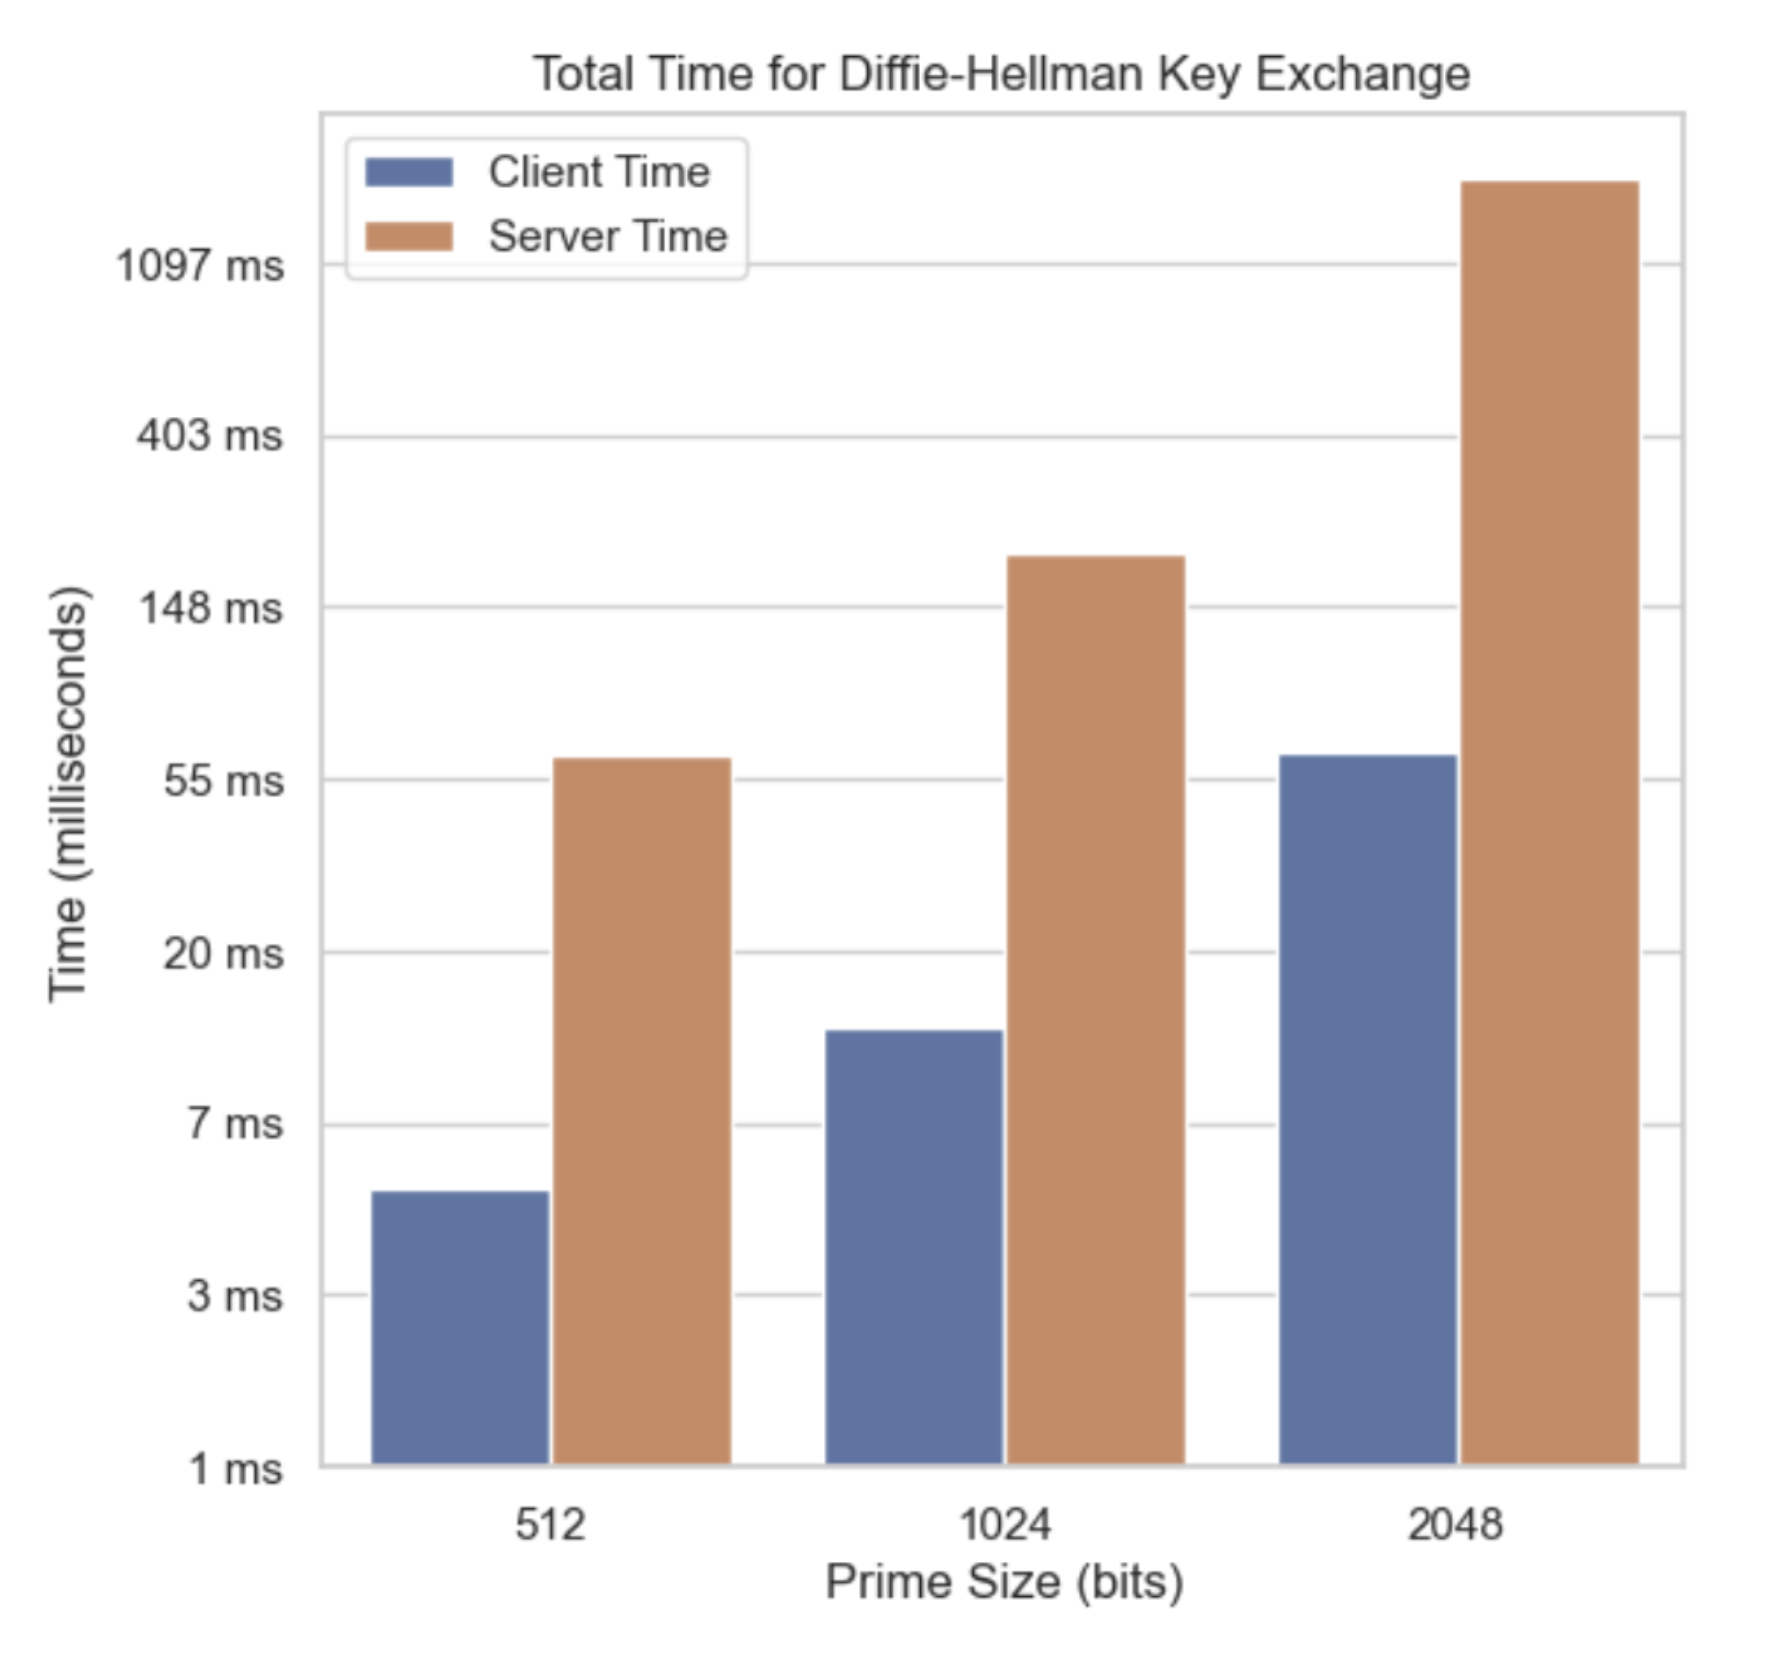
\includegraphics[width=0.7\linewidth]{dh_1.png}
    \caption{The total time in milliseconds the Diffie-Hellman key exchange takes depending on the size of the prime number. Note that the y-axis is logged, which means the server takes significantly longer time to set up. This is due to the fact that the server is the one generating the shared prime number, which is done at the server set up phase. }
    \label{fig:Time to Crack Diffie-Hellman Key Exchange}
\end{figure}

\subsection{Advanced Encryption Standard (AES)}
As mentioned before, IKEv2 specifically uses AES-256, which uses a 256 bit key and a total of 14 rounds. AES begins with what’s known as key expansion; intuitively, it expands the key to its desired 256 bits and creates 15 different round keys (one for initialization and one for each round). Naturally, the details are significantly more nuanced and complex, which have been omitted in this paper, so, for further details, refer to here. \cite{improved_aes} Next, it arranges the 128-bit packet in row-major order with one transformed byte in each of the 16 squares, where a transformed byte is defined by combining said byte with a round key through a bitwise XOR. Canonical, this XOR operation is known as the AddRoundKey operation because XOR is the add operation of the finite field. After this initial setup, AES starts its first round.\\
\\
For AES-256 and IKEv2, there are 4 operations per round and 14 total rounds.\\
\\
The first operation is known as SubBytes, and, as the name suggests, substitutes every byte through a substitution box or S-box, which is just a nonlinear vectorial boolean function. \cite{generalities_vectorial} Additionally, the substitutions come with two rules: 1. there are no fixed points (a byte can not substitute with itself), and 2. there are no opposite fixed points (a byte can not substitute with a bitflip of itself). Note that the S-box is just a table look up, so the entire process is very efficient.\\
\\
The next operation, ShiftRows, is also intuitively very straightforward. Simply, do not move the first row and shift the second, third, and fourth row by one, two, and three to the left, respectively, while looping back around.\\
\\
Similarly, AES also mixes the columns, which is canonically known as MixColumns. Using a 4x4 matrix and multiplying each column by said matrix, the result is four new columns where each new byte is a linear combination of the old bytes of their original column. To undo such a transformation in the decryption stage, the algorithm uses the inverse matrix, so it's important that our 4x4 transformation matrix is invertible. (An additional comment is that, on the last round, the MixColumns operation is not run as it would not have any effect on the final code).
\\
Finally, to finish off the round, AddRoundKey is applied again, resulting in a 128 bit block of seemingly gibberish. Perform these rounds thirteen more times, and the result is AES. The final output of the last round’s AddRoundKey will be what is sent over the channel for the server or client to decrypt.\\
\\
The 128-bit cypher has never been broken before, and the 256 bit cypher is approximately $340 \times 10^{36}$ times more difficult to crack. \cite{aes_study}
\begin{figure}[h]
    \centering
    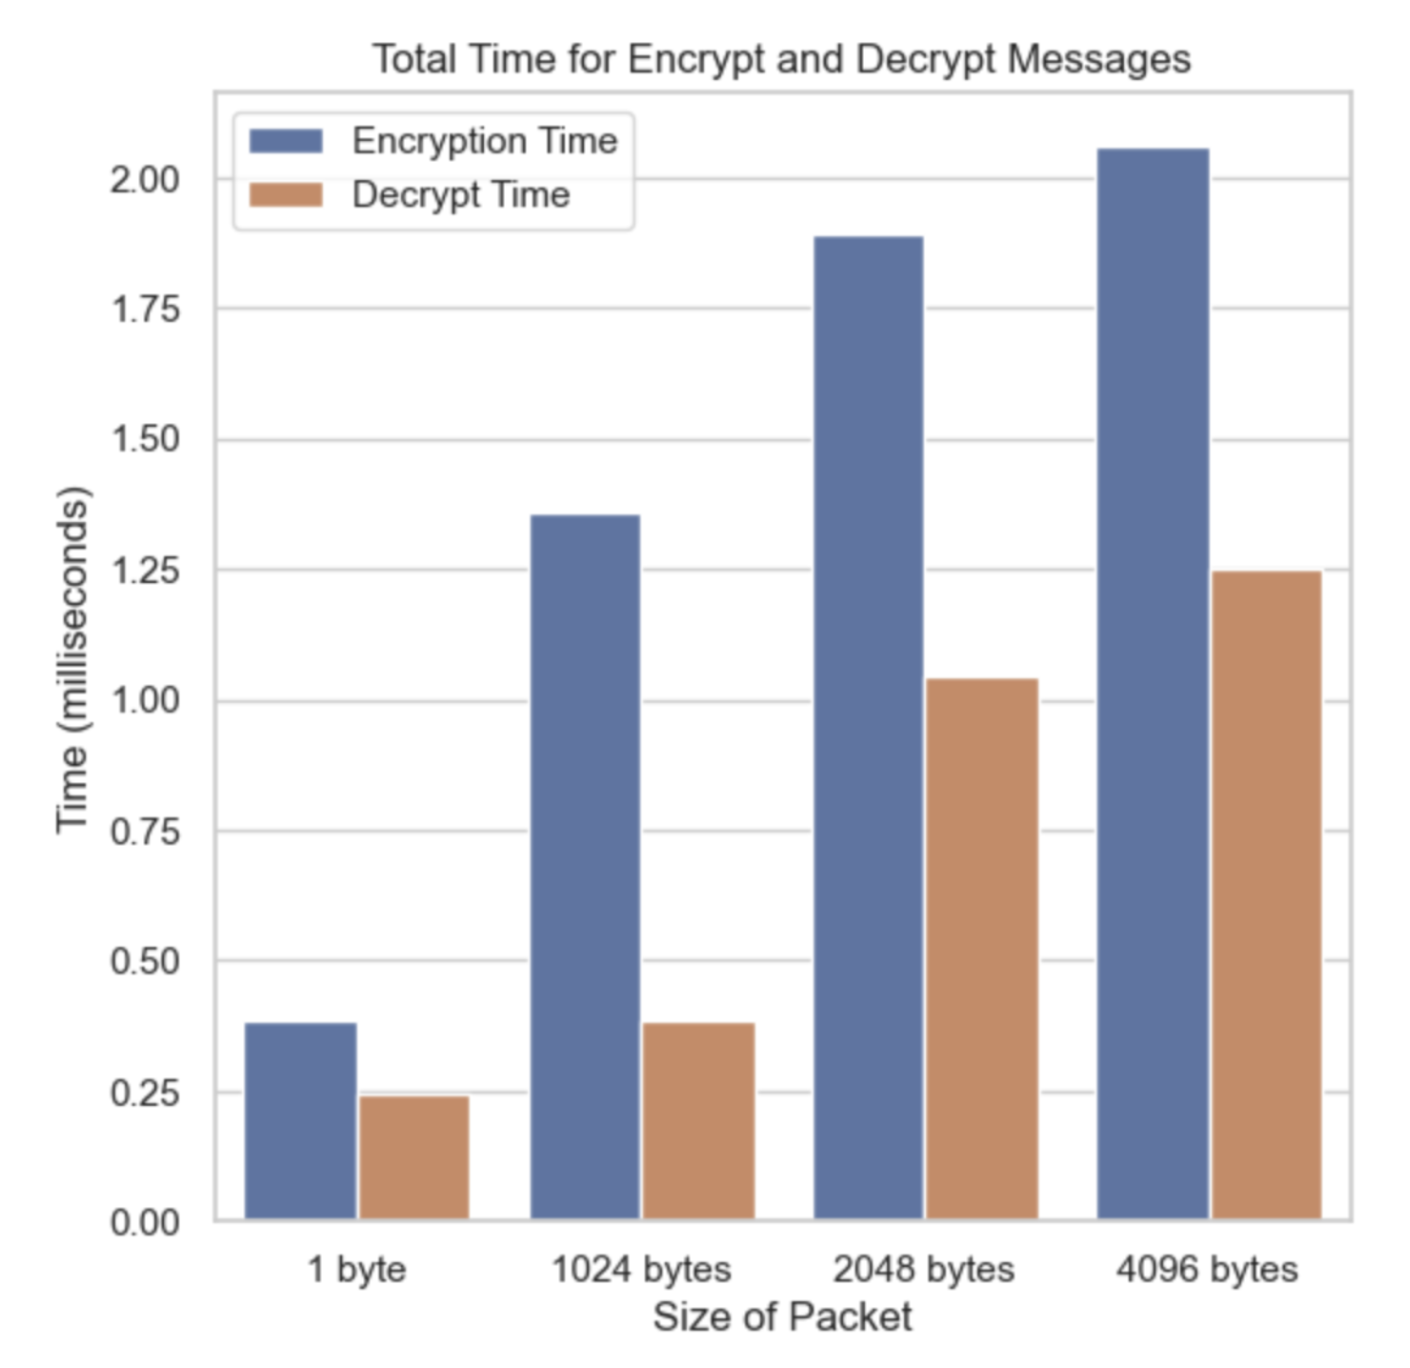
\includegraphics[width=0.7\linewidth]{aes_1.png}
    \caption{The total time in milliseconds AES to encrypt and decrypt messages. These extremely quick speeds are due to the fact that AES operations are built into modern day CPUs.}
    \label{fig:Time for Encryption and Decryption using AES}
\end{figure}

\section{Analysis}
\subsection{Security}
IKEv2 is renowned for its robust security features, employing advanced cryptographic algorithms (AES-256) and mutual authentication mechanisms. In contrast, PPTP is considered less secure due to vulnerabilities such as outdated encryption methods.
\subsection{Performance}
IKEv2 typically offers superior performance compared to PPTP, primarily due to its support for multi-threading and faster tunnel establishment. PPTP, while efficient in terms of bandwidth utilization, may suffer from latency issues and slower connection speeds, especially in high-traffic environments.
\subsection{Compatibility}
IKEv2 has gained support from modern operating systems and network equipment. PPTP has broad compatibility across various platforms and devices, including legacy systems and is generally considered to be more compatible with systems.
\subsection{Ease of Implementation}
PPTP is often favored for its simplicity in configuration and deployment, making it suitable for small-scale deployments. Conversely, IKEv2 may require more effort for setup, but offers greater flexibility and scalability for complex network infrastructures.
\subsection{Overall}
In summary, IKEv2 stands out for its robust security, superior performance, and growing compatibility with modern systems and equipment. While PPTP remains widely compatible and easy to implement, its security vulnerabilities and potential performance issues make it less favorable for certain use cases, particularly those requiring high levels of security and performance. Therefore, the choice between IKEv2 and PPTP ultimately depends on the specific requirements and priorities of the deployment scenario.
\section{Appendix: Implementation Details}
For our analysis, we implemented both PPTP and IKEv2 protocols. Our work is available at:
\underline{\url{https://github.com/jessetyao/VPNProj}}.

\newpage

\bibliographystyle{splncs04}
\bibliography{bibliography}

\end{document}
